\documentclass[11pt]{article}

% ---- packages -------------------------------------------------------------
\usepackage[margin=1in]{geometry}
\usepackage{amsmath,amssymb,amsthm,mathtools}
\usepackage{tikz}
\usetikzlibrary{arrows.meta,positioning,fit,backgrounds,calc,shapes.geometric}
\usepackage[hidelinks]{hyperref}

% ---- theorem environments -------------------------------------------------
\theoremstyle{plain}
\newtheorem{theorem}{Theorem}
\newtheorem{proposition}[theorem]{Proposition}
\newtheorem{corollary}[theorem]{Corollary}
\newtheorem{lemma}[theorem]{Lemma}
\theoremstyle{definition}
\newtheorem{definition}[theorem]{Definition}

% ---- notation -------------------------------------------------------------
\newcommand{\Aut}{\mathcal{A}}
\newcommand{\Soft}{\mathcal{S}}
\newcommand{\St}{\sigma}
\newcommand{\ext}{\mathsf{ext}}
\newcommand{\der}{\mathsf{der}}
\newcommand{\val}{\mathsf{val}}
\newcommand{\basis}{\mathsf{basis}}
\newcommand{\reduces}{\longrightarrow}
\newcommand{\reducesu}{\longrightarrow_{u}}
\newcommand{\Facts}{\mathsf{Fact}}
\newcommand{\confff}{\theta}
\newcommand{\irule}[3]{\dfrac{\begin{array}{c}#2\end{array}}{#3}\;\;\textsc{(#1)}}

% poisoning-ablation numbers (filled from the run)
\newcommand{\PoisonON}{\text{--}}
\newcommand{\PoisonOFF}{\text{--}}
\newcommand{\PoisonTrue}{\text{--}}

% ---- tikz styles ----------------------------------------------------------
\tikzset{
  store/.style={draw, rounded corners, minimum width=3.1cm, minimum height=1.15cm,
                align=center, font=\small, thick},
  gate/.style={draw, diamond, aspect=2, inner sep=1pt, align=center,
               font=\scriptsize, thick, fill=black!5},
  flow/.style={-{Stealth[length=2mm]}, thick},
  softflow/.style={-{Stealth[length=2mm]}, thick, dashed},
  lbl/.style={font=\scriptsize, align=center}
}

\title{\textbf{Systemic Epistemic Governance}\\[2pt]
\large Deriving a Proposition versus the Authority to Persist and Act on It:\\
An Operational Semantics for Provenance-Gated Admission in Persistent Cognitive Systems}

\author{Stefan Ragland\\ Dominion Labs\\ \texttt{research@dmnlabs.org}}
\date{\today}

\begin{document}
\maketitle

\begin{abstract}
A persistent cognitive system must decide, continuously, which of its own
inferences may change its long-term state. We argue for a single principle:
\emph{a system should distinguish the ability to derive a proposition from the
authority to persist and act upon it, and that distinction can be enforced as a
system-wide state-transition invariant.} We call the resulting discipline
\emph{systemic epistemic governance} (SEG). SEG partitions persistent state into
an \emph{authoritative tier}---the store the reasoner treats as authorized and
the rules permitted to act---writable only through provenance admission or
\emph{independent} validation, and a \emph{soft tier} of beliefs, derivations,
and generalizations that materializes automatically and is, by construction,
non-authoritative and volatile. We give a small-step operational semantics for
SEG and prove four \emph{structural} guarantees---authoritative provenance-%
rootedness, non-circular promotion, execution safety, and soft-tier
non-authority---together with a separation result, \emph{non-autonomous
authoritative escalation}: under SEG no amount of internal derivation can move an
error into authority without a fresh qualifying promotion, whereas the uniform
auto-materialization discipline of prior architectures lets a single error
escalate without bound. The guarantees are deliberately true \emph{by
construction}, in the sense of type-system and information-flow safety; the
contribution is a construction that makes specific epistemic failures
unreachable. We are explicit that the promotion condition we enforce is
\emph{syntactic} independence, and we lay out the stronger independence notions,
a threat model, and an ablation program that a full empirical validation
requires, reporting first governance-on/off measurements.
\end{abstract}

% ===========================================================================
\section{Introduction}
% ===========================================================================

An intelligent system that persists---that accumulates knowledge across time
rather than restarting each episode---faces a control problem a stateless
predictor never does: \emph{what may write to persistent state?} Every inference
produces a candidate belief. If those candidates flow automatically into the
store the system later reasons from, the system can generalize and grow, but it
inherits a well-known amplification loop: inference writes memory, future
inference consumes that memory, and errors, once written, seed further errors and
reinforce themselves. If instead nothing is admitted without external
adjudication, the system is safe but inert.

This paper is organized around one principle, which we state plainly and then
enforce formally:
\begin{quote}\itshape
Persistent cognitive systems should distinguish the ability to \emph{derive} a
proposition from the \emph{authority} to persist and act upon it, and that
distinction can be enforced as a system-wide state-transition invariant.
\end{quote}
We call the discipline that enforces it \emph{systemic epistemic governance}
(SEG). SEG does not attach a confidence score to beliefs and leave the semantics
of persistence unchanged; it changes that semantics. In SEG a fact may
\emph{exist}---be stored, reasoned over, reinforced, and generalized from---while
being \emph{prohibited} from becoming authoritative, from being returned as
authoritative, or from triggering an action, unless it is promoted. Concretely
(Figure~\ref{fig:arch}), persistent state is split into an \emph{authoritative
tier} $\Aut$---the relational store the reasoner treats as authorized and the
rules permitted to act---and a \emph{soft tier} $\Soft$---beliefs, derived
conclusions, induced generalizations, consolidated schemas. Writes to $\Aut$ are
hard-gated (external provenance, or promotion through \emph{independent}
validation); the soft tier materializes automatically, is provenance-stamped, is
never returned as authoritative, and decays without reinforcement.

We are careful about the word \emph{authoritative}: it denotes what the system is
\emph{permitted to treat} as authorized, not what is objectively true. A trusted
source or an independent validation can be wrong; SEG governs epistemic
authorization, not metaphysical truth.

SEG sits at the intersection of three mature disciplines
(Figure~\ref{fig:map}): \emph{truth maintenance} (why a belief is held),
\emph{data provenance} (how a datum was derived), and \emph{authorization and
information-flow control} (what a component is permitted to do). Its contribution
is to make \emph{epistemic authority itself a first-class, system-wide transition
invariant}, rather than a property of a single reasoning store, a metadata tag,
or a runtime hope. The metatheory is intentionally \emph{structural}: as with
type soundness or capability safety, the guarantees are not emergent properties
of a learned system but invariants enforced by the admissible transitions---an
ill-formed epistemic move is simply not a step of the system.

\paragraph{Contributions.}
(1) An operational semantics for SEG (\S\ref{sec:state}--\S\ref{sec:sem});
(2) four structural guarantees and a \emph{non-autonomous escalation} separation
theorem (\S\ref{sec:meta}), with an explicit hierarchy of independence notions
distinguishing what is enforced from what is assumed;
(3) a realization in a running architecture, a threat model, and a falsifiable
ablation program with first measurements (\S\ref{sec:impl}--\S\ref{sec:empirical}).

\begin{figure}[t]
\centering
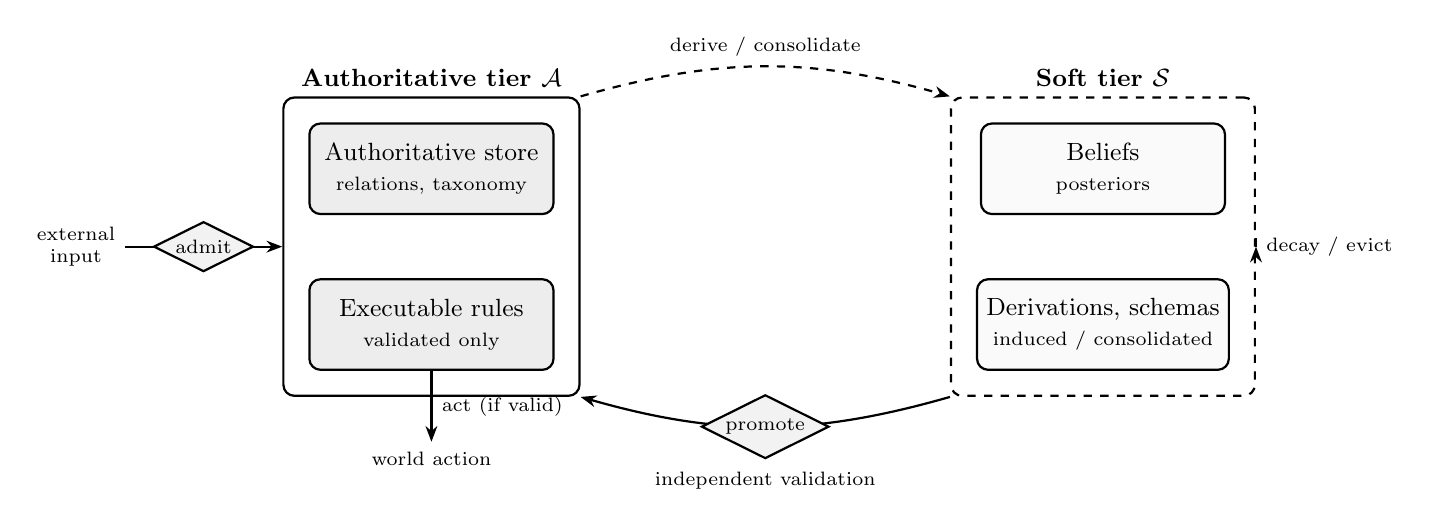
\begin{tikzpicture}[node distance=0.9cm]
  \node[store, fill=black!7] (cg) {Authoritative store\\ \scriptsize relations, taxonomy};
  \node[store, fill=black!7, below=0.8cm of cg] (rules) {Executable rules\\ \scriptsize validated only};
  \node[draw, thick, rounded corners, fit=(cg)(rules), inner sep=9pt,
        label={[font=\small\bfseries]above:Authoritative tier $\Aut$}] (Abox) {};
  \node[store, right=5.4cm of cg, fill=black!2] (beliefs) {Beliefs\\ \scriptsize posteriors};
  \node[store, below=0.8cm of beliefs, fill=black!2] (schemas) {Derivations, schemas\\ \scriptsize induced / consolidated};
  \node[draw, thick, dashed, rounded corners, fit=(beliefs)(schemas), inner sep=9pt,
        label={[font=\small\bfseries]above:Soft tier $\Soft$}] (Sbox) {};
  % external admission gate on the arrow
  \node[left=2.0cm of Abox, font=\scriptsize, align=center] (ext) {external\\ input};
  \draw[flow] (ext) -- node[gate,midway]{admit} (Abox.west);
  % derive / consolidate (top) : auth -> soft
  \draw[softflow] (Abox.north east) to[bend left=16]
        node[above, lbl]{derive / consolidate} (Sbox.north west);
  % promote (bottom) : soft -> auth, gate ON the arrow
  \draw[flow] (Sbox.south west) to[bend left=16]
        node[gate, midway, fill=black!5] (prg){promote} (Abox.south east);
  \node[below=1pt of prg, lbl]{independent validation};
  % decay self-loop on soft
  \draw[softflow] (Sbox.east) to[out=25,in=-25,looseness=5]
        node[right, lbl]{decay / evict} (Sbox.east);
  % act
  \node[below=0.9cm of rules, font=\scriptsize] (act){world action};
  \draw[flow] (rules) -- node[right, lbl]{act (if valid)} (act);
\end{tikzpicture}
\caption{Systemic epistemic governance. External input reaches $\Aut$ only
through a provenance \emph{admission gate}. Reasoning and consolidation write
\emph{automatically} into $\Soft$ (dashed). Soft content becomes authoritative
only through the \emph{promotion gate}, which requires evidence \emph{independent}
of the content's own derivation basis. Only validated rules in $\Aut$ may act;
soft content decays absent reinforcement.}
\label{fig:arch}
\end{figure}

% ===========================================================================
\section{Related Work}
\label{sec:related}
% ===========================================================================

SEG lies at the confluence of three literatures (Figure~\ref{fig:map}). We
position it against each, taking care not to caricature the systems it builds on.

\paragraph{Truth maintenance and belief revision.} Justification- and
assumption-based truth-maintenance systems attach justifications to beliefs and
perform dependency-directed retraction~\cite{doyle1979,dekleer1986}. AGM belief
revision axiomatizes rational change of a belief set under new
information~\cite{agm1985}; default and nonmonotonic logics reason defeasibly with
revisable conclusions~\cite{reiter1980}; epistemic logic formalizes what an agent
knows versus believes~\cite{fhmv1995}. SEG shares the commitment to tracking why a
belief is held and to revisability, and its promotion gate is a descendant of
dependency reasoning. It differs by operating over an \emph{entire persistent
cognitive system} rather than one reasoning store, by materializing a soft tier
automatically and marking it explicitly non-authoritative, and by requiring
promotion evidence \emph{independent of a conclusion's own support}---a condition
a TMS records dependencies for but does not, in general, enforce.

\paragraph{Data provenance and integrity.} Provenance semirings and lineage
systems track how tuples are derived through query
evaluation~\cite{green2007,cheney2009}; database integrity constraints restrict
admissible states~\cite{ahv1995}. This machinery governs \emph{data}; SEG applies
an analogous discipline to \emph{cognitive state}, where the governed quantity is
which self-generated beliefs may become authoritative and actionable.

\paragraph{Authorization and information-flow control.} Lattice models of secure
information flow~\cite{denning1976}, decentralized label models~\cite{myers1997},
and language-based information-flow security~\cite{sabelfeld2003} enforce, by
construction, that data of one clearance cannot influence another; runtime
assurance architectures gate a complex controller behind a verified safety
monitor~\cite{sha2001}. SEG is, in this lineage, an \emph{epistemic} access-control
discipline: promotion is a clearance boundary, and \emph{execution safety}
(\S\ref{sec:meta}) is the epistemic analogue of ``untrusted code cannot act.''
To our knowledge, treating epistemic authority as a system-wide flow invariant
over a cognitive architecture's persistent state is not covered by these lines
individually.

\paragraph{Cognitive architectures and agent memory.} SEG is a persistent
cognitive architecture. NARS unifies inference and control under insufficient
knowledge and resources; crucially, its beliefs are \emph{revisable summaries of
experience}, not immutable axioms, and inference writes revisable judgments back
into memory~\cite{wang2013}. The OpenCog/CogPrime programme and its Hyperon
successor pursue emergence through cognitive synergy over a shared Atomspace whose
Atoms carry truth \emph{and} attention values and support transient values,
contexts, and multiple spaces~\cite{goertzel2014,goertzel2023}; MeTTa gives its
operational semantics of metagraph rewriting~\cite{meredith2023}. Psi-theoretic
architectures organize cognition through needs and global
modulators~\cite{bach2015}. We do \emph{not} claim these systems lack provenance,
uncertainty, contexts, or revision. Our claim is narrower and, we think, more
defensible: in these architectures derived content and admitted content share a
store and become available to the system on the same footing, whereas SEG makes
\emph{epistemic authority} a categorical, system-wide transition invariant---a
derived proposition is representationally present but epistemically unauthorized
until promoted. Modern LLM-agent memory systems (retrieval with source tracking;
long-term memory managers~\cite{park2023,packer2023}) attach provenance and
recency to stored text but likewise do not impose an authority boundary between
derived and admitted content. SEG is compatible with the Common Model of
Cognition's decomposition~\cite{laird2017}; it adds a governance discipline over
what that decomposition may persist and act upon.

\begin{figure}[t]
\centering
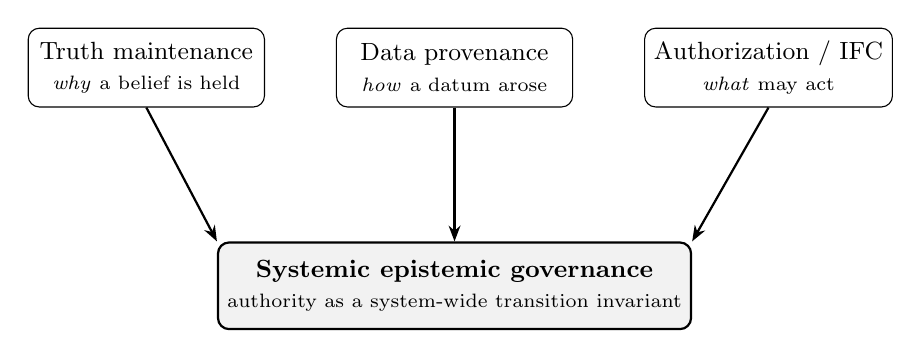
\begin{tikzpicture}[every node/.style={font=\small}]
  \node[draw,rounded corners,align=center,minimum width=3.0cm,minimum height=1.0cm] (tms){Truth maintenance\\ \scriptsize\emph{why} a belief is held};
  \node[draw,rounded corners,align=center,minimum width=3.0cm,minimum height=1.0cm,right=0.9cm of tms] (prov){Data provenance\\ \scriptsize\emph{how} a datum arose};
  \node[draw,rounded corners,align=center,minimum width=3.0cm,minimum height=1.0cm,right=0.9cm of prov] (auth){Authorization / IFC\\ \scriptsize\emph{what} may act};
  \node[draw,thick,fill=black!5,rounded corners,align=center,minimum width=5.6cm,minimum height=1.1cm,below=1.7cm of prov] (seg){\textbf{Systemic epistemic governance}\\ \scriptsize authority as a system-wide transition invariant};
  \draw[flow] (tms.south) -- (seg.north west);
  \draw[flow] (prov.south) -- (seg.north);
  \draw[flow] (auth.south) -- (seg.north east);
\end{tikzpicture}
\caption{SEG as the intersection of three disciplines: it inherits
justification/revision from truth maintenance, lineage from provenance, and gated
influence from authorization/information-flow control, and adds a system-wide
authority invariant over persistent cognitive state.}
\label{fig:map}
\end{figure}

% ===========================================================================
\section{The Epistemic State}
\label{sec:state}
% ===========================================================================

Fix a set $\Facts$ of \emph{facts}, ranged over by $f,g$; facts include
relational atoms $r(a,b)$ and \emph{rules} $\rho$ (guarded actions
$\gamma \Rightarrow \alpha$). A \emph{provenance} record is one of
\[
  \pi ::= \ext(s) \mid \der(\Gamma) \mid \val(E),
\]
where $s$ is an external source with a nonempty root-evidence envelope,
$\Gamma \subseteq \Facts$ is a \emph{derivation basis} (the premises an inference
used), and $E \subseteq \Facts$ is a \emph{validation evidence set}. We write
$\basis(\der(\Gamma)) = \Gamma$.

\begin{definition}[Epistemic state]
An epistemic state is a pair $\St = \langle \Aut, \Soft\rangle$ where the
\emph{authoritative tier} $\Aut \subseteq \Facts \times \{\ext(\cdot),
\val(\cdot)\}$ carries only external or validated justifications, and the
\emph{soft tier} $\Soft \subseteq \Facts \times [0,1] \times \{\der(\cdot)\}$
holds soft facts $(f,\confff,\der(\Gamma))$ with confidence $\confff$ and a
derivation record. $\St$ is \emph{well-formed} if every $(f,\pi)\in\Aut$ has
$\pi\in\{\ext(\cdot),\val(\cdot)\}$.
\end{definition}

A rule $\rho\in\Aut$ with $\val(\cdot)$ is \emph{executable}; a rule present only
in $\Soft$ is a \emph{candidate}.

\paragraph{Auxiliary judgments.} The semantics uses four side judgments, kept
abstract so that concrete systems may instantiate them: $\Gamma \vdash f : \confff$
(``an inference licenses $f$ at confidence $\confff$ from premises $\Gamma$'');
$\mathsf{confirms}(E,f)$ (``$E$ supports $f$''); $\mathsf{denies}(\Aut,f)$
(``$\Aut$ contains an admitted denial of $f$''); and
$\mathsf{upd}(\confff_g,\confff_f)$ (a confidence-revision function). The
metatheory below is parametric in these judgments: it constrains \emph{where} and
\emph{under what admission condition} facts may be written, not \emph{how}
confidence is computed.

% ===========================================================================
\section{Operational Semantics}
\label{sec:sem}
% ===========================================================================

We give a small-step relation $\St \reduces \St'$ (Figure~\ref{fig:rules}).

\begin{figure}[t]
\footnotesize
\begin{gather*}
\irule{Admit}{\text{external source } s \text{ presents } f \text{ with root envelope } e}
  {\langle \Aut,\Soft\rangle \reduces \langle \Aut\cup\{(f,\ext(s,e))\},\ \Soft\rangle}
\\[9pt]
\irule{Derive}{\Gamma \subseteq \Aut\cup\Soft \\ \Gamma \vdash f \;:\; \confff}
  {\langle \Aut,\Soft\rangle \reduces \langle \Aut,\ \Soft\cup\{(f,\confff,\der(\Gamma))\}\rangle}
\\[9pt]
\irule{Propagate}{(f,\confff_f,\_)\in\Soft \\ (g,\confff_g,d)\in\Soft \\ \confff_g' = \mathsf{upd}(\confff_g,\confff_f)}
  {\langle \Aut,\Soft\rangle \reduces \langle \Aut,\ \Soft[(g,\confff_g,d)\mapsto(g,\confff_g',d)]\rangle}
\\[9pt]
\irule{Promote}{(f,\confff,\der(\Gamma))\in\Soft \\ E\cap\Gamma=\emptyset \\
   \mathsf{confirms}(E,f) \\ \neg\,\mathsf{denies}(\Aut,f)}
  {\langle \Aut,\Soft\rangle \reduces \langle \Aut\cup\{(f,\val(E))\},\ \Soft\rangle}
\\[9pt]
\irule{Decay}{(f,\confff,d)\in\Soft \\ \confff' = \confff+(\confff_0-\confff)(1-e^{-\lambda\Delta t})}
  {\langle \Aut,\Soft\rangle \reduces \langle \Aut,\ \Soft[(f,\confff,d)\mapsto(f,\confff',d)]\rangle}
\\[9pt]
\irule{Evict}{(f,\confff,d)\in\Soft \\ |\confff-\confff_0|<\varepsilon \\ \mathsf{evidence}(f)<k}
  {\langle \Aut,\Soft\rangle \reduces \langle \Aut,\ \Soft\setminus\{(f,\confff,d)\}\rangle}
\\[9pt]
\irule{Query}{q \text{ asked}}
  {\langle \Aut,\Soft\rangle \reduces \langle \Aut,\Soft\rangle \;\text{(answer tier-tagged)}}
\\[9pt]
\irule{Act}{\rho=(\gamma\Rightarrow\alpha) \\ (\rho,\val(E))\in\Aut \\ \gamma \text{ holds}}
  {\langle \Aut,\Soft\rangle \reduces \langle \Aut,\Soft\rangle \;\text{(world action } \alpha)}
\end{gather*}
\caption{Small-step operational semantics for SEG. \textsc{Admit} and
\textsc{Promote} are the only rules that write $\Aut$; \textsc{Derive},
\textsc{Propagate}, \textsc{Decay}, \textsc{Evict} act only on $\Soft$;
\textsc{Query} and \textsc{Act} do not modify the epistemic state. The
independence side-condition $E\cap\Gamma=\emptyset$ in \textsc{Promote} is the
core governance premise.}
\label{fig:rules}
\end{figure}

Two commitments are visible in the rules. First, \textsc{Derive} and
\textsc{Propagate}---the automatic activity of a reasoner---target only $\Soft$.
Second, the sole path from $\Soft$ to $\Aut$, \textsc{Promote}, requires evidence
\emph{disjoint from the fact's own derivation basis}.

\paragraph{What ``independent'' means, precisely.} The disjointness condition
$E\cap\Gamma=\emptyset$ is \emph{syntactic}, and we do not overstate it. We
distinguish four strengthening notions:
\begin{description}
\item[L1 (syntactic).] $E\cap\Gamma=\emptyset$: the confirming set shares no fact
with the derivation basis. \emph{This is what Figure~\ref{fig:rules} enforces and
what \S\ref{sec:meta} proves over.}
\item[L2 (provenance).] $E$ and $\Gamma$ share no upstream source or lineage root.
\item[L3 (statistical).] Observations in $E$ are not correlated repetitions of
those in $\Gamma$ (same measurement, same model).
\item[L4 (adversarial).] $E$ is not manufactured to appear independent while
sharing a hidden common cause with $\Gamma$.
\end{description}
L1 does not imply L2--L4: two syntactically distinct facts may share a source,
dataset, measurement error, or poisoned model. The guarantees below hold at L1;
we treat L2--L4 as the deployment obligation and the object of the threat model
(\S\ref{sec:threat}). Where the running system approximates a stronger level (by
collapsing observations of a common causal lineage before they count as evidence;
\S\ref{sec:empirical}) we say so.

% ===========================================================================
\section{Metatheory}
\label{sec:meta}
% ===========================================================================

A state is \emph{reachable} if $\St_0 \reduces^{*} \St$ for a well-formed $\St_0$
whose authoritative tier is $\ext$-justified. The results are \emph{structural
invariants}: as in type-system soundness and information-flow control, their value
is that the corresponding failures are unreachable by any admissible transition,
not that they are surprising. We say so plainly, and treat the simplicity of the
proofs as the point.

\begin{theorem}[Authoritative provenance-rootedness]
\label{thm:root}
For every reachable $\langle\Aut,\Soft\rangle$ and every $(f,\pi)\in\Aut$,
$\pi=\ext(\cdot)$ or $\pi=\val(\cdot)$; no authoritative fact carries a derivation
justification.
\end{theorem}
\begin{proof}
Induction on the length of $\St_0\reduces^{*}\St$. Base: $\Aut_0$ is
$\ext$-justified. Step: only \textsc{Admit} (adding $\ext$) and \textsc{Promote}
(adding $\val$) write $\Aut$; \textsc{Derive}/\textsc{Propagate} write $\Soft$;
the remaining rules do not add to $\Aut$. The invariant is preserved.
\end{proof}

\begin{lemma}[Well-formedness preservation]
\label{lem:wf}
If $\St$ is well-formed and $\St\reduces\St'$ then $\St'$ is well-formed.
\end{lemma}
\begin{proof}
Immediate from Theorem~\ref{thm:root}'s step analysis: every write to $\Aut$
carries $\ext$ or $\val$; writes to $\Soft$ preserve its shape.
\end{proof}

\begin{theorem}[Non-circular promotion]
\label{thm:noncirc}
If a \textsc{Promote} step admits $(f,\val(E))$ where $f$'s soft record is
$\der(\Gamma)$, then $E\cap\Gamma=\emptyset$. No fact attains authority on
evidence drawn from its own derivation basis.
\end{theorem}
\begin{proof}
Immediate from the premise of \textsc{Promote}.
\end{proof}

\begin{theorem}[Execution safety]
\label{thm:exec}
A world action occurs only if its rule $\rho$ satisfies $(\rho,\val(E))\in\Aut$.
No candidate or purely derived rule ever acts.
\end{theorem}
\begin{proof}
\textsc{Act} is the only world-effecting rule and requires $(\rho,\val(E))\in\Aut$.
By Theorem~\ref{thm:root} a rule in $\Aut$ is $\ext$- or $\val$-justified; a
$\der$-justified rule lives only in $\Soft$ and cannot match.
\end{proof}

\begin{theorem}[Soft-tier non-authority and volatility]
\label{thm:soft}
Let $(f,\confff,\der(\Gamma))\in\Soft$ with $f\notin\Aut$. Then \emph{(a)} $f$ is
never returned as authoritative by \textsc{Query} (answers are tier-tagged;
authoritative answers range over $\Aut$); and \emph{(b)} absent any
\textsc{Promote} of $f$ or reinforcement, iterated \textsc{Decay} drives
$\confff\to\confff_0$ and \textsc{Evict} removes $f$.
\end{theorem}
\begin{proof}
(a) by the tier-tagging of \textsc{Query}; (b) \textsc{Decay} contracts toward
$\confff_0$, after which \textsc{Evict} applies.
\end{proof}

The four invariants combine into the separation that motivates the discipline.
We name it for what it guarantees---not general error containment, but the
prohibition of \emph{autonomous} escalation of an error into authority.

\begin{proposition}[Non-autonomous authoritative escalation]
\label{prop:escalation}
Let $e$ be an erroneous fact in $\Soft$. \emph{(i)} No sequence of
\textsc{Derive} and \textsc{Propagate} steps ever adds an $e$-derived fact to
$\Aut$; any authoritative appearance of such a fact requires a \textsc{Promote}
step supplying $E$ with $E\cap\Gamma=\emptyset$ and $\mathsf{confirms}(E,\cdot)$.
\emph{(ii)} In the uniform variant $\reducesu$, in which \textsc{Derive} writes
$\Aut$ directly, for every $n$ there is a reachable state containing $n$ distinct
authoritative errors derived from the single error $e$.
Thus under $\reduces$ derivation alone cannot escalate an error into authority,
whereas under $\reducesu$ it does so without bound.
\end{proposition}
\begin{proof}
(i) By Theorem~\ref{thm:root}, $\Aut$ never gains a $\der$-justified fact;
\textsc{Derive}/\textsc{Propagate} touch only $\Soft$, so the sole channel into
$\Aut$ is \textsc{Promote}, whose premise is as stated. (ii) Under $\reducesu$,
from $e\in\Aut$ apply \textsc{Derive} to obtain $e'\in\Aut$ (basis $\{e\}$), then
$e''\in\Aut$ (basis $\{e'\}$), and so on; after $n$ steps $\{e',\dots,e^{(n)}\}$
are $n$ distinct authoritative errors.
\end{proof}

\begin{corollary}[Contamination bound at L1]
\label{cor:bound}
Under $\reduces$, the number of erroneous facts in $\Aut$ is at most the number of
\textsc{Promote} steps whose (L1-independent) evidence incorrectly confirms an
error. \emph{This bound is only as strong as the independence actually enforced:}
at L1 it constrains autonomous internal escalation (Prop.~\ref{prop:escalation})
but not poisoning by correlated sources engineered to satisfy $E\cap\Gamma=
\emptyset$ (an L4 attack; \S\ref{sec:threat}).
\end{corollary}

We regard Proposition~\ref{prop:escalation}(i) as the transferable content: an
internal error can propagate arbitrarily within $\Soft$ yet cannot, by derivation
alone, cross into authority; crossing requires a fresh qualifying event.
Figure~\ref{fig:cascade} contrasts the two disciplines.

\begin{figure}[t]
\centering
\resizebox{\textwidth}{!}{%
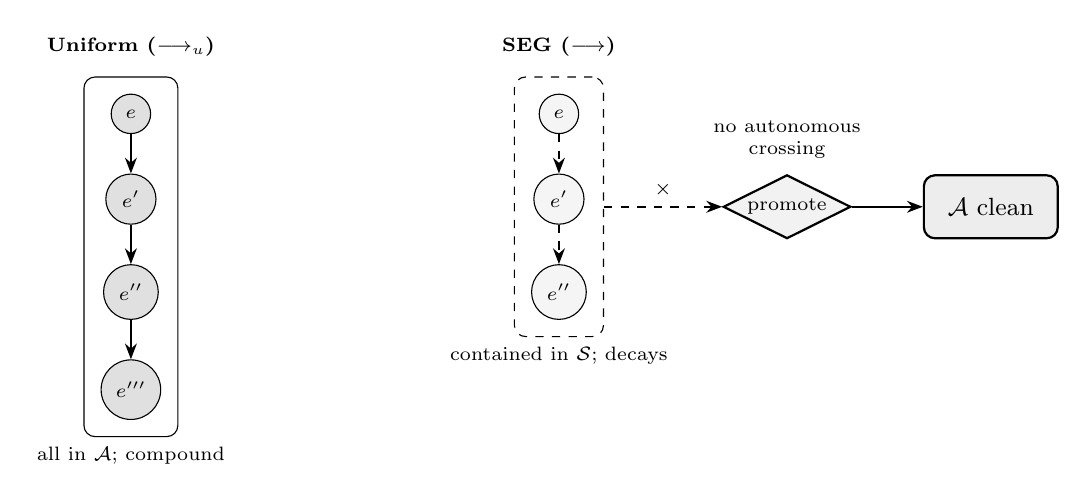
\begin{tikzpicture}[node distance=0.5cm and 2.6cm, every node/.style={font=\scriptsize}]
  % uniform: vertical error chain, all authoritative
  \node[font=\scriptsize\bfseries] (utitle) {Uniform ($\reducesu$)};
  \node[draw, circle, fill=black!12, below=0.35cm of utitle] (e0){$e$};
  \node[draw, circle, fill=black!12, below=of e0] (e1){$e'$};
  \node[draw, circle, fill=black!12, below=of e1] (e2){$e''$};
  \node[draw, circle, fill=black!12, below=of e2] (e3){$e'''$};
  \draw[flow](e0)--(e1); \draw[flow](e1)--(e2); \draw[flow](e2)--(e3);
  \node[draw, rounded corners, fit=(e0)(e1)(e2)(e3), inner sep=6pt,
        label={[font=\scriptsize]below:all in $\Aut$; compound}] {};
  % SEG: chain contained in soft, blocked at promotion
  \node[font=\scriptsize\bfseries, right=3.4cm of utitle] (stitle){SEG ($\reduces$)};
  \node[draw, circle, fill=black!4, below=0.35cm of stitle] (s0){$e$};
  \node[draw, circle, fill=black!4, below=of s0] (s1){$e'$};
  \node[draw, circle, fill=black!4, below=of s1] (s2){$e''$};
  \draw[softflow](s0)--(s1); \draw[softflow](s1)--(s2);
  \node[draw, dashed, rounded corners, fit=(s0)(s1)(s2), inner sep=6pt,
        label={[font=\scriptsize]below:contained in $\Soft$; decays}] (sbox){};
  \node[gate, right=1.5cm of sbox] (g){promote};
  \node[store, minimum width=1.7cm, minimum height=0.8cm, fill=black!7,
        right=0.9cm of g] (aut){$\Aut$ clean};
  \draw[softflow] (sbox.east) -- node[above, font=\scriptsize]{$\times$} (g);
  \draw[flow] (g) -- (aut);
  \node[above=2pt of g, font=\scriptsize, align=center]{no autonomous\\ crossing};
\end{tikzpicture}%
}
\caption{Non-autonomous escalation (Prop.~\ref{prop:escalation}). Left: under
$\reducesu$ one authoritative error is a valid basis for further authoritative
errors, which compound without bound. Right: under $\reduces$ errors and their
derivations remain in $\Soft$, decay, and cannot cross into $\Aut$ by derivation
alone; crossing requires a fresh promotion supplying independent evidence.}
\label{fig:cascade}
\end{figure}

% ===========================================================================
\section{Threat Model}
\label{sec:threat}
% ===========================================================================

The semantics is clean under cooperative assumptions; persistent systems are not
deployed under them. We state what the current model does and does not protect,
so that the guarantees are not read beyond their scope. Table~\ref{tab:threat}
maps threat classes to the level at which SEG, as formalized here, addresses them.

\begin{table}[t]
\centering
\small
\begin{tabular}{l l}
\hline
Threat & Status in the present model\\
\hline
Internal inference cascade & Structurally prevented (Prop.~\ref{prop:escalation})\\
Circular reinforcement into authority & Structurally prevented (Thms.~\ref{thm:root},\ref{thm:noncirc})\\
Correlated evidence (repeated measurements) & Partially addressed; L3, mechanism-level (\S\ref{sec:empirical})\\
Source compromise & Not formally modeled\\
Provenance forgery & Not formally modeled\\
Adversarial fabricated independence (L4) & Acknowledged limitation of L1 promotion\\
Validator error / miscalibration & Not formally modeled\\
\hline
\end{tabular}
\caption{Threat classes vs.\ protection in the formalized model. SEG's structural
guarantees concern autonomous internal escalation and circular reinforcement; the
promotion boundary is only as strong as the independence it enforces, and
source/validator/forgery threats require the stronger independence levels
(L2--L4) as future formal work.}
\label{tab:threat}
\end{table}

% ===========================================================================
\section{Realization and Reproducibility}
\label{sec:impl}
% ===========================================================================

SEG is the persistence discipline of a running cognitive architecture (Lyric), a
Python system over a relational (PostgreSQL) store. We summarize the
correspondence; the metatheory of \S\ref{sec:meta} is the intended invariant of
these mechanisms, and we are careful \emph{not} to present the implementation as a
validation of the robustness hypothesis (\S\ref{sec:empirical}).

\paragraph{Authoritative tier.} The relational store (a typed, polarity-bearing
concept graph) is written through a single ingress requiring an evidence envelope
with provenance and root evidence; there is no direct-write path, and content
\emph{derived} internally (e.g.\ by an analogy process) is admitted only as
\emph{derivative}, never as a root---the realization of \textsc{Admit} and
Theorem~\ref{thm:root}. Executable authority for learned rules is separated from
their existence: an induced rule persists as a non-executable \emph{candidate} and
becomes executable only through a validation step requiring held-out evidence
\emph{disjoint from its induction basis} that refuses to validate on any
contradiction---the realization of \textsc{Promote}, its L1 side-condition, and
\textsc{Act}'s gate.

\paragraph{Soft tier.} Reasoning conclusions, hypotheses, induced schemas,
analogical mappings, and consolidated generalizations materialize automatically
into belief and schema stores, provenance-stamped but ungated; belief posteriors
relax toward a non-committal point and are evicted absent reinforcement---the
realization of \textsc{Derive}, \textsc{Propagate}, \textsc{Decay}, \textsc{Evict}.

\paragraph{Reproducibility caveats.} Provenance envelopes are stored rows linking
each fact to its evidence and source type; derivation lineage is the recorded
basis set. Lineage tracking is therefore an additional write per admission (a
measurable but here unquantified overhead). Independence at the belief level is
approximated by collapsing observations that share a causal lineage before they
count as evidence (an L3 approximation). Concurrency is not modeled formally:
simultaneous promotion attempts on related facts are serialized by the store, and
a formal treatment of promotion races is future work. We describe a correspondence
between model and system, not a from-scratch reproducible artifact; accordingly we
present the implementation as a \emph{realization}, and rest the paper's settled
claims on the model and its guarantees.

% ===========================================================================
\section{A Falsifiable Robustness Hypothesis}
\label{sec:empirical}
% ===========================================================================

Proposition~\ref{prop:escalation} predicts a measurable difference between SEG and
uniform auto-materialization; the same system can be run with a governance gate
disabled, isolating a single variable. We state the hypothesis and are explicit
that current evidence demonstrates \emph{mechanisms behaving as specified}, not
yet the architecture-level claim.

\begin{quote}\itshape
Holding the cognitive architecture fixed and changing only the admission
discipline measurably changes authoritative contamination, false-action rate, and
post-correction consistency, at a quantifiable cost in generalization latency.
\end{quote}

\noindent\textbf{First measurements (governance on/off, one variable).}
Table~\ref{tab:ablation} reports the soft tier's independence-collapse rule: with
it disabled, $k$ mutually-correlated confirmations of one claim drive its posterior
from $0.998$ ($k{=}3$) to $1.000$ ($k{=}5$); enabled, they collapse to a single
grounding and the posterior stays $0.724$ for all $k$---the circular-reinforcement
failure bounded. Separately, the conversational admission gate declines assertions
the authoritative tier refutes: on a stream of five store-refuted and five
novel-consistent assertions, all five refuted were declined and all five novel
retained; notably the refuted assertions stayed excluded even with the
conversational gate bypassed, because an ingress-level provenance/polarity check
independently declines contradictory admissions---a layered governance we did not
fully ablate. These illustrate the mechanisms at work, not the full hypothesis.

\begin{table}[t]
\centering
\small
\begin{tabular}{c c c}
\hline
$k$ correlated confirmations & independence \textsc{on} & \textsc{off}\\
\hline
1 & 0.724 & 0.724\\
3 & 0.724 & 0.998\\
5 & 0.724 & 1.000\\
\hline
\end{tabular}
\caption{Governance on/off, one variable. Posterior assigned to a claim after $k$
mutually-correlated confirmations (identical causal lineage), with the soft
tier's independence-collapse rule enabled vs.\ disabled. Independence handling
bounds confidence; without it correlated evidence inflates the posterior toward
certainty---the circular-reinforcement failure the discipline is designed to
contain.}
\label{tab:ablation}
\end{table}

\noindent\textbf{The ablation program.} A systems-grade validation runs the full
battery, governance \textsc{on}/\textsc{off}:
\begin{enumerate}
\item \emph{Error-cascade injection} --- inject one authoritative-looking false
premise; measure downstream authoritative contamination over time. Directly tests
Prop.~\ref{prop:escalation}. \emph{(Priority next step.)}
\item \emph{Correlated poisoning} --- multiple sources that appear distinct but
share a causal origin; test whether the independence mechanism catches them. This
attacks the L1$\to$L4 gap (\S\ref{sec:threat}) and is the decisive experiment for
the weakest assumption.
\item \emph{Correction propagation} --- correct a fact after downstream
derivation; measure stale beliefs and time to consistency.
\item \emph{Action safety} --- a candidate rule made highly supported internally
but false; measure whether the ablated system acts and SEG refuses. Empirical
counterpart of Theorem~\ref{thm:exec}.
\item \emph{Generalization latency / Pareto frontier} --- quantify the cost of
governance: how much responsiveness is traded for integrity. The interesting
question is not whether gates raise integrity (they do) but the
integrity/generalization frontier.
\end{enumerate}
A null or negative result---no authoritative-integrity advantage, or a prohibitive
generalization cost---would disconfirm the discipline's value and is an outcome we
regard as informative.

% ===========================================================================
\section{Discussion}
% ===========================================================================

SEG is a position about \emph{where} to place a barrier in a persistent cognitive
system, made precise as a transition invariant. Its guarantees are structural and
modest by design: they say what the authoritative tier can and cannot contain, in
the sense that type safety says what a well-typed program cannot do. The
interesting empirical question---whether the containment the metatheory guarantees
translates into robustness that matters, and at what cost to generalization---is
left open on purpose, with the ablation battery to settle it. The load-bearing
contribution is the distinction itself: a proposition may be derivable without
being authorized to persist or act, and that authorization can be a first-class,
system-wide invariant. Provenance, promotion, decay, and containment are the
machinery that enforces it. The principal open problems are the stronger
independence notions (L2--L4) and a threat model that formalizes source
compromise, provenance forgery, and validator error, so that the promotion
boundary is robust not only to autonomous internal escalation but to evidence
engineered to defeat it.

% ===========================================================================
\section{Conclusion}
% ===========================================================================

We introduced systemic epistemic governance: the principle that a persistent
cognitive system should separate the ability to derive a proposition from the
authority to persist and act upon it, enforced as a system-wide transition
invariant. We gave its operational semantics and proved four structural
guarantees and a non-autonomous escalation separation, distinguishing carefully
the syntactic independence we enforce from the stronger notions a robust
deployment needs. The discipline is realized in a running architecture, and it
yields a falsifiable prediction distinguishing it from uniform auto-materialization.
Whether that prediction holds, and what it costs, is the experiment the model was
built to make precise.

\begin{thebibliography}{99}
\small
\bibitem{doyle1979} J.~Doyle. A truth maintenance system. \emph{Artificial
Intelligence}, 12(3):231--272, 1979.
\bibitem{dekleer1986} J.~de~Kleer. An assumption-based TMS. \emph{Artificial
Intelligence}, 28(2):127--162, 1986.
\bibitem{agm1985} C.~Alchourr\'on, P.~G\"ardenfors, D.~Makinson. On the logic of
theory change: partial meet contraction and revision functions. \emph{J.\ Symbolic
Logic}, 50(2):510--530, 1985.
\bibitem{reiter1980} R.~Reiter. A logic for default reasoning. \emph{Artificial
Intelligence}, 13(1--2):81--132, 1980.
\bibitem{fhmv1995} R.~Fagin, J.~Y.~Halpern, Y.~Moses, M.~Y.~Vardi. \emph{Reasoning
About Knowledge}. MIT Press, 1995.
\bibitem{green2007} T.~J.~Green, G.~Karvounarakis, V.~Tannen. Provenance
semirings. In \emph{PODS}, 2007.
\bibitem{cheney2009} J.~Cheney, L.~Chiticariu, W.-C.~Tan. Provenance in databases:
why, how, and where. \emph{Foundations and Trends in Databases}, 1(4), 2009.
\bibitem{ahv1995} S.~Abiteboul, R.~Hull, V.~Vianu. \emph{Foundations of
Databases}. Addison-Wesley, 1995.
\bibitem{denning1976} D.~E.~Denning. A lattice model of secure information flow.
\emph{Communications of the ACM}, 19(5):236--243, 1976.
\bibitem{myers1997} A.~C.~Myers, B.~Liskov. A decentralized model for information
flow control. In \emph{SOSP}, 1997.
\bibitem{sabelfeld2003} A.~Sabelfeld, A.~C.~Myers. Language-based information-flow
security. \emph{IEEE J.\ Selected Areas in Communications}, 21(1), 2003.
\bibitem{sha2001} L.~Sha. Using simplicity to control complexity. \emph{IEEE
Software}, 18(4):20--28, 2001.
\bibitem{wang2013} P.~Wang. \emph{Non-Axiomatic Logic: A Model of Intelligent
Reasoning}. World Scientific, 2013.
\bibitem{goertzel2014} B.~Goertzel. \emph{Engineering General Intelligence}
(the CogPrime architecture). Atlantis Press, 2014.
\bibitem{goertzel2023} B.~Goertzel et~al. OpenCog Hyperon: a framework for AGI at
the human level and beyond. \emph{arXiv:2310.18318}, 2023.
\bibitem{meredith2023} L.~G.~Meredith, B.~Goertzel, J.~Warrell, A.~Vandervorst.
Meta-MeTTa: an operational semantics for MeTTa. \emph{arXiv:2305.17218}, 2023.
\bibitem{bach2015} J.~Bach. Modeling motivation in MicroPsi~2. In \emph{AGI}, 2015.
\bibitem{park2023} J.~S.~Park et~al. Generative agents: interactive simulacra of
human behavior. In \emph{UIST}, 2023.
\bibitem{packer2023} C.~Packer et~al. MemGPT: towards LLMs as operating systems.
\emph{arXiv:2310.08560}, 2023.
\bibitem{laird2017} J.~E.~Laird, C.~Lebiere, P.~S.~Rosenbloom. A standard model of
the mind. \emph{AI Magazine}, 38(4), 2017.
\end{thebibliography}

\end{document}
